\paragraph{The Human Brain Project} is a European Flagship that is developing a European research infrastructure advancing brain research, medicine, and brain-inspired information technology for both industry and science.
The project is now entering its third phase, with over 100 partnering institutions from over 20 countries in Europe, as well as over 100 partnering projects.
There are 12 subprojects in HBP that span the development of six ICT-based Platforms.
One of these six platforms is the Neuromorphic Computing (NMC) Platform, with two systems;
the mixed-signal VLSI BrainScaleS (Brain-inspired multiScale computation in neuromorphic hybrid systemS) and the massively parallel digital SpiNNaker (Spiking Neural Network architecture \cite{amunts_human_2016}.

\paragraph{The main applicaiton} of BrainScaleS is the study of physical neural dynamics at a higher rate than available in biology.
Thus, BrainScaleS was designed with a speed-up factor for 1000 - 10 000 compared to biological wall time.
Modeling of biological neurons and synapses are realized with physical, analog components, while the interconnections are digital and programmable to increase efficiency \cite{zoschke_full_2017}.
In addition to brain research, this neuromorphic system may enable new applications in robotics, artificial intelligence, and human-machine interfaces.
Using a physical model keeps a one-to-one relationship between the neurons and synapses of the biological example and the model,
preserving the fault tolerance concerning the loss, which is inherent in the biological brain.

\paragraph{The power- and material costs} when simulating the neuron is reduced by several orders of magnitude by using only a few analog components per neuron, compared to several million involved in the same task while solving these equations numerically in a microprocessor core.
\cite{schemmel_wafer-scale_2010}
As the neurons on the HICANN chip are emulated with analog electronics rather than with a high number of arithmetic operations, the circuitry is power-efficient, and a complete HICANN consumes only $1.3 W/cm^2$.
The theoretical worst-case power consumption of a wafer module is 2 kW.
\cite{zoschke_full_2017}


\paragraph{The current BrainScaleS implementation} is at the Kirchhoff-Institute for Physics at Heidelberg University, enables up to 20 wafer modules, with up to 200 000 neurons and 40 000 000 synapses, per wafer.
Wafer-Scale integration was chosen to allow for the extreme bandwidth requirements of the accelerated system \cite{zoschke_full_2017}.
The Wafer-Scale integration is partly following the proposal of C. Mead, who proposed interconnecting chips with analog components by integrating the production wafer \cite{mead_neuromorphic_1990}.
The base chips on the BrainScaleS wafer are the HICANN, \vref{sect:hicann}.
A single 200 mm wafer carries 384 HICANN chips. Equipped to the wafer is FPGAs that handle communication with other wafers and with the host computer.
In addition to delivering signals to and from each wafer, the FPGAs are used to configure the chips. \cite{zoschke_full_2017}.
On one wafer module, there are 48 FPGAs, each equipped with Gigabit-Ethernet, to handle the high amount of event data per time that will occur on the accelerated system.
12 Gigabit connections are routed to each edge of the module, respectively, to communicate with other wafer modules and the host computer.
On the wafer, one FPGA controls 8 HICANN chips that together account for one reticle.
Every HICANN has two full-duplex serial LVDS links with separate clock and data lines to the FPGA module, and each link is capable of transmitting two GBit/s.
One fundamental concept with the HICANN is that it allows the construction of neurons with over 10 000 pre-synaptic connections.
The high connectivity leads to a transmission requirement of 1.4 GEvents/s per neuron, which is why the silicon wafer is kept as a whole to produce shorter transmission lines and a lower capacitive load.
\cite{zoschke_full_2017}

\subsubsection{The Neuron Model}\label{sect:adexp} at the basis of the HICANN is called the Adaptive Exponential Integrate-and-Fire model (AdExp) \cite{brette_adaptive_2005}.
The AdExp model was co-developed by the FACETS project \cite{schemmel_wafer-scale_2010}, a predecessor to the BranScaleS project, which is now part of the NMC platform of HBP.
The model contains several additions compared to the standard Integrate-and-Fire model (IAF):
\begin{equation}\label{eq:adexp-membrane}
-C_m\frac{dV}{dt} = g_l(V-E_l) - g_l\Delta_{th}exp(\frac{V-V_{th}}{\Delta_{th}}) + g_e(t)(V-E_e)+g_l(t)(V-E_i)+w(t)
\end{equation}
The variables $C_m, g_l E_l, E_e$ and $E_i$ are the membrane capacity, the leakage conducatance and the leakage, exciatory and inhibitory reversal potentials.
The variables $g_e(t)$ and $g_i(t)$ represent the total excitatory and inhibitory synaptic conductances.
The introduced addition to the standard IAF model is the \textit{exponential} term on the right-hand side of the equation, which models the near-asymptotic growth of the membrane potential under certain conditions.
The \textit{treshold potential} $V_{th}$ represents the critical value above which this rapid growth can occur, and the \textit{slope factor} $\Delta_{th}$ determines the rapidness of the triggered growth.
Such a situation is interpreted as a spike, and each time a spike is detected, a separately generated output event signal is transmitted to possible connected target neurons or recording devices, and the membrane potential is forced to a reset potential $V_{reset}$ by an adjustable reset conductance.
A second equation describes the temporal evolution of the socalled \textit{adaption current} $w(t)$:
\begin{equation}\label{eq:adexp-adaption}
-\tau_{w}\frac{dw}{dt} = w(t) - a(V-E_l)
\end{equation}
Every time a spike is emitted by the neuron, $w$ changes its value: $w \rightarrow w + b$.
The time constant and the efficacy of the so-called \textit{sub-treshold} adaption mechanism are given by $\tau_w$ and $a$, while $b$ defines the amount of so-called \textit{spike-triggered} adaption.
The exponential term of equation \ref{eq:adexp-membrane} and the adaption function of equation \ref{eq:adexp-adaption} can be deactivated to reduce the AdExp model to the standard IAF model.
\cite{schemmel_wafer-scale_2010}\cite{brette_adaptive_2005}

\cref{fig:adexp-circuit} shows the individual circuit components and \cref{fig:adexp-firing} illustrates the firing modes of this neuron circuit.
In the currently effective implementation of BrainScaleS, BSS-1, the neurons are implemented in a 180 mm CMOS technology.
By design, the system is scalable with newer generations of CMOS technology and HICANN chips \cite{zoschke_full_2017}.
Millner et al.  \cite{millner_vlsi_2010} describes the hardware implementation of the neuron to great detail. The paper
also report that the emulation of an IAF neuron with the implemented hardware is 3000 times more power-efficient and accelerated by a factor of 10 000 when compared to an Izhikevich neuron simulated on a supercomputer \cite{millner_vlsi_2010}.
The Izhikevich neuron is a popular model because it gives an accurate representation of a neuron's functionality while being simple to model \cite{schuman_survey_2017}.

\begin{figure}  \centering
  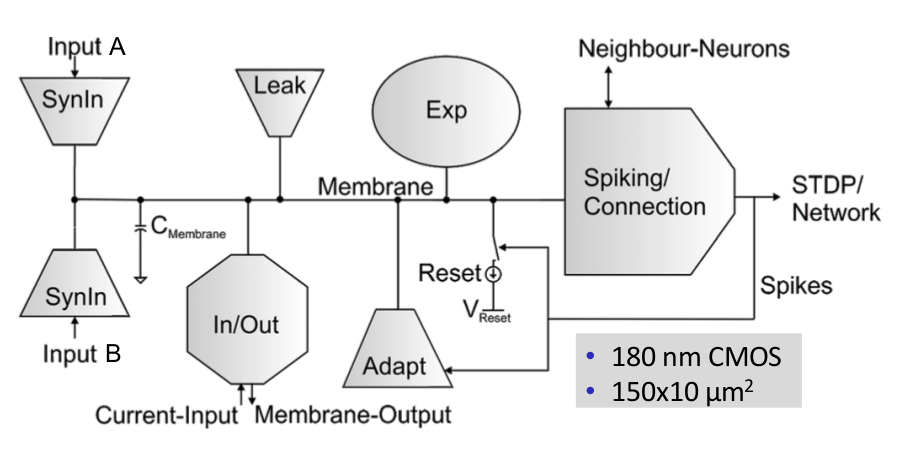
\includegraphics[width=.8\textwidth]{adexp-circuit}
    \label[figure]{fig:adexp-circuit}
    \captionof{figure}{Schematic diagram of the AdExp neuron circuit, taken from \cite{schemmel_wafer-scale_2010}.}
\end{figure}%
\begin{figure}  \centering
  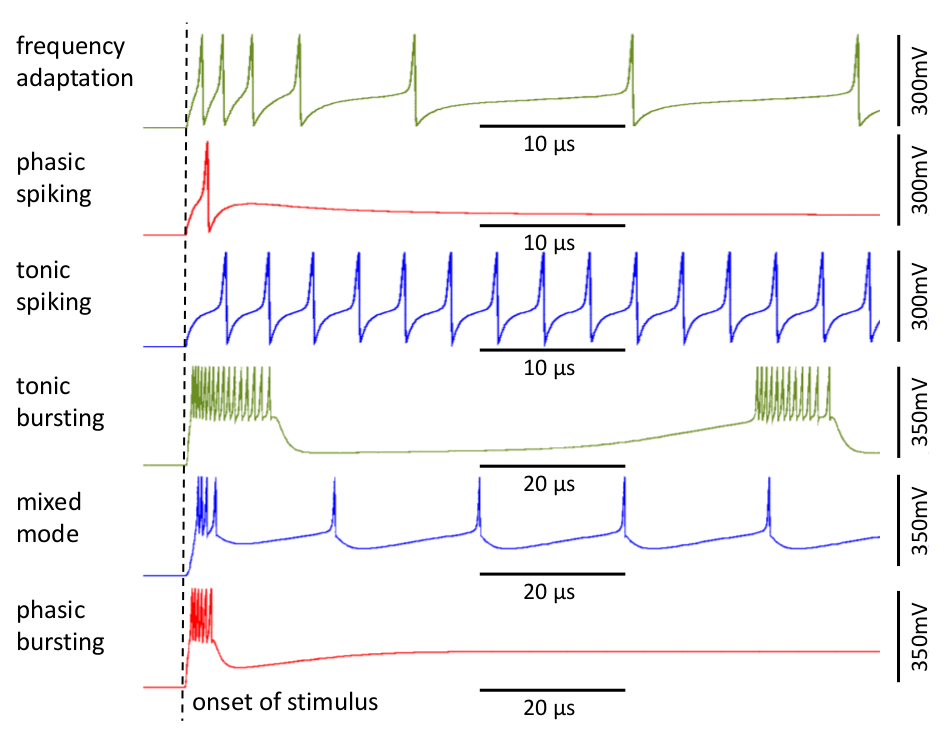
\includegraphics[width=.9\textwidth]{adexp-firing}
    \label[figure]{fig:adexp-firing}
    \captionof{figure}{Example of firing modes of the AdExp neuron circuit, taken from \cite{schemmel_wafer-scale_2010}.}
\end{figure}

\subsubsection{Communication} on a wafer happens on several levels; There is the communication happening between the local neurons and synapses, then there are Layer 1 (L1) and Layer 2 (L2) channels depending on how far the communication reaches.
This subsection discusses the inter-neuron communication of the system in terms of how closely it models nature, which is vital information for any comparison analysis - for example, involving Integrated Information Theory, \vref{sect:iit}.

\paragraph{The composing structure} of the neurons, with their respective synapses, is called the Analog Network Core (ANC), shown in \cref{fig:anc}.
The neurons are constructed by Dendrite Membrane (DenMem) circuits that allow neurons with up to 14336 synaptic inputs per neuron.
The synaptic weights, stored in a four-bit SRAM, are represented by a current generated by a DAC.
Short-Term Depression (STD) and Spike-Timing Dependent Plasticity (STDP) are implemented by the use of capacitors modulating the signals and by an algorithm that manipulates the digitally stored weights.
\cref{fig:synapse} shows a schematic diagram of the synaptic circuit, where $g_max$ is a programmable analog parameter controlling the scale of the DAC.
In each ANC, communication is asynchronous and mixed-signal.
The cores are highly integrated systems working in a continuous-time mode.
\cite{schemmel_wafer-scale_2010}

\begin{figure}  \centering
  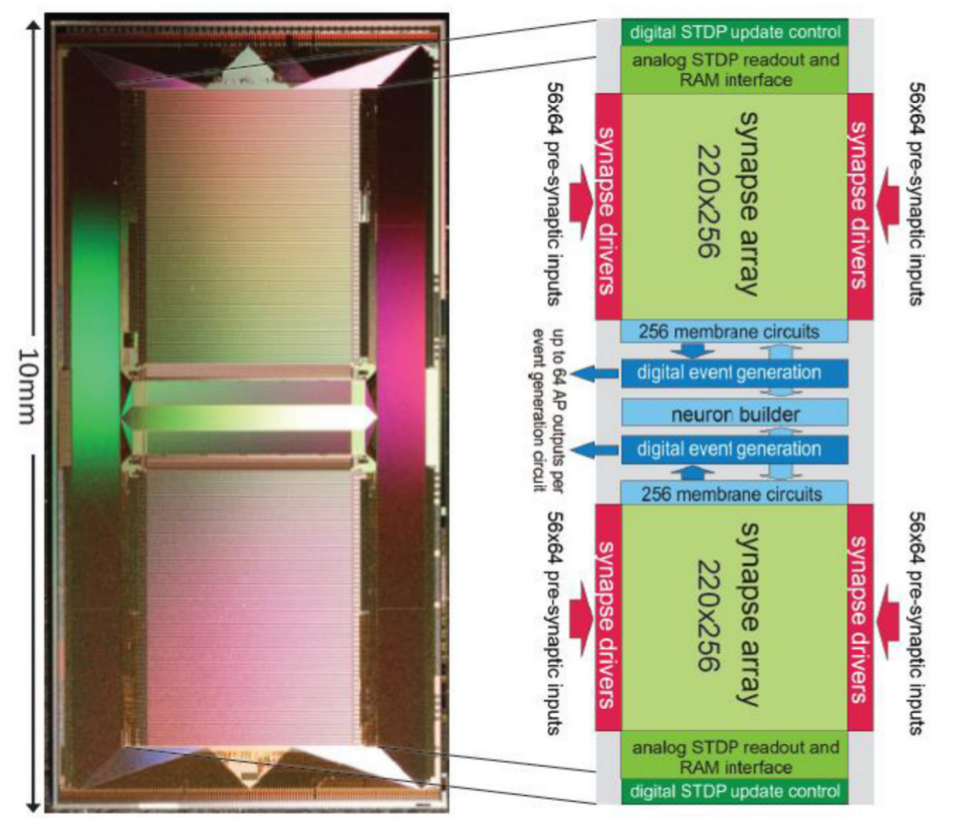
\includegraphics[width=.8\textwidth]{anc-diagram}
  \label[figure]{fig:anc}
  \captionof{figure}{To the left is a single HICANN chip, and to the right is diagram of the ANC which is located at the center of the chip, taken from \cite{thakur_large-scale_2018}.}
\end{figure}
\begin{figure}  \centering
  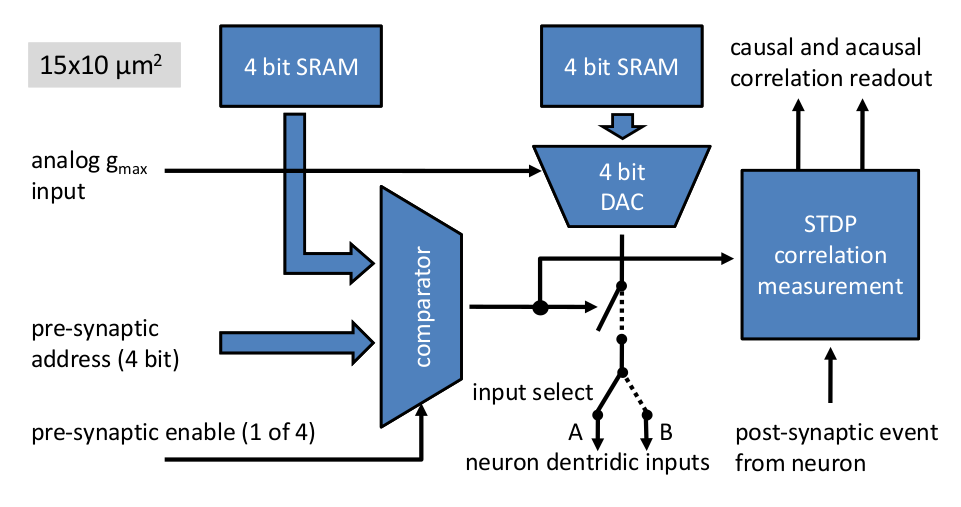
\includegraphics[width=.8\textwidth]{synapse-circuit}
  \label[figure]{fig:synapse}
  \captionof{figure}{Schematic diagram of a synapse circuit, taken from \cite{schemmel_wafer-scale_2010}.}
\end{figure}

\paragraph{The communication protocol} between ANCs is L1, a real-time serial event protocol operating at up to 2 Gb/s.
The protocol uses two time-frame bits and six address data bits and uses continuous-time transmission \cite{schemmel_wafer-scale_2008}.
This digital transmission protocol limits power consumption while retaining continuous communication. \cite{schemmel_wafer-scale_2010}.
Wafer-Scale integration was selected to support the channel density requirements of an accelerated system, where each neuron can receive over 10k pre-synaptic inputs  \cite{schemmel_wafer-scale_2010}.
The solution of the Wafer-Scale integration is explained in detail in \cite{zoschke_full_2017} and \cite{thakur_large-scale_2018}.
The inter-ANC communication on a wafer is real-time, serial, and only dependent on the states of the local circuits involved.

Each HICANN chip has an L2 channel to allow for inter-wafer communication.
Due to latency issues involved with real-time long-range communication, L2 is based on packets-switching and digitized time stamps \cite{schemmel_wafer-scale_2010} \cite{thakur_large-scale_2018}.
This digital communication in-between wafers, or with the host computer, is handled by FPGAs \cite{zoschke_full_2017}.
Therefore, inter-neuron communication between wafers has a lower level of integration.
